\documentclass[format=acmlarge,10pt,screen,nonacm,natbib=false]{acmart}
\usepackage{geometry}

\if 0
\setlength\paperheight{11in}
\setlength\paperwidth{8.5in}
\setlength{\textwidth}{7in}
\setlength{\textheight}{9.25in}
\setlength{\oddsidemargin}{-.25in}
\setlength{\evensidemargin}{-.25in}

\fi

%
\usepackage{xspace}
\usepackage{multirow}
\usepackage{comment}
\usepackage{fancybox, fancyvrb, calc}
\usepackage{subcaption}
\usepackage[inline]{enumitem}
\usepackage{amsmath, amssymb}
\usepackage{cite,url}
\usepackage{pbox}
\usepackage{balance}
\usepackage{wrapfig}
%
%\usepackage[T1]{fontenc}
\usepackage[utf8]{inputenc}
\usepackage{mathptmx}
\usepackage{enumitem}
\setlist{nolistsep}
\usepackage{hhline}
%
\captionsetup[table]{skip=-1pt,font={footnotesize}}
\captionsetup[subfigure]{skip=-1pt,font={footnotesize}}
\captionsetup[figure]{font={footnotesize}}
\Urlmuskip=0mu plus 1mu
\hypersetup{%
  colorlinks=true,      % false: boxed links; true: colored links
  linkcolor=blue,       % color of internal links
  citecolor=magenta,    % color of links to bibliography
  filecolor=cyan,       % color of file links
  urlcolor=blue          % color of external links
}
%
\usepackage{leading}
\leading{12pt}
%
\usepackage{minted}
\usepackage{listings}
\lstset{
  columns=flexible,
  mathescape,
  keepspaces=true,
  escapeinside={(*}{*)},
  basicstyle=\ttfamily\small  
}
%
%\usepackage[subtle]{savetrees}
\usepackage[small,compact]{titlesec}
\usepackage{outlines}
%
\newcommand{\cut}[1]{}
%
\newcommand{\paragraphnone}[1]{\vspace{0.075in}\noindent{\bf #1}}
\newcommand{\paragrapha}[1]{\vspace{0.075in}\noindent{\bf #1.}}
\newcommand{\paragraphq}[1]{\vspace{0.075in}\noindent{\bf #1}}
%
\newcommand{\eg}{e.g., }
\newcommand{\etc}{{etc.}\xspace}
\newcommand{\ie}{i.e., }
\newcommand{\ccp}{CCP\xspace}
%
\newcommand{\an}[1]{{\color{green}\bf AN: {#1}}}
\newcommand{\sn}[1]{{\color{purple}\bf NG: {#1}}}
\newcommand{\hb}[1]{{\color{brown}\bf HB: {#1}}}
\newcommand{\ma}[1]{{\color{red}\bf MA: {#1}}}
\newcommand{\pg}[1]{{\color{blue}\bf PG: {#1}}}
\newcommand{\fc}[1]{{\color{blue}\bf FC: {#1}}}
\newcommand{\dr}[1]{{\color{magenta}\bf DR: {#1}}}
\newcommand{\radhika}[1]{{\color{cyan}\bf RM: {#1}}}
%
\newcommand{\datapath}{datapath\xspace}
\newcommand{\datapaths}{datapaths\xspace}
\newcommand{\Datapaths}{Datapaths\xspace}
\newcommand{\Datapath}{Datapath\xspace}
%
\frenchspacing
%
\newcommand{\handlers}{callbacks\xspace}
\newcommand{\userspace}{user-space\xspace}
\newcommand{\kernelspace}{kernel-space\xspace}
%
\newcommand{\controller}{agent\xspace}

\newcommand{\ct}[1]{{\tt #1}}
\newcommand{\ngs}[1]{{\textcolor{red}{NG: #1}}}
\newcommand{\Para}[1]{\vspace{4pt}\noindent{\bf #1}}
\newcommand{\Sec}[1]{\S\ref{#1}}


\begin{document}
%\begin{textblock}{13.5}(1,0.5)\fcolorbox{black}{gray!7!}{
%\begin{minipage}{\dimexpr\textwidth-2\fboxsep-2\fboxrule\relax}
%    \centering
%    \scriptsize
%    The version of this paper published at SIGCOMM 2018 contained a labelling error in Figure 10. This has been corrected in this version.
%\end{minipage}}
%\end{textblock}

\title{Corrigendum: Restructuring Endpoint Congestion Control}
\author{Akshay Narayan}
\author{Frank Cangialosi}
\author{Deepti Raghavan}
\author{Prateesh Goyal}
\author{Srinivas Narayana}
\author{Radhika Mittal} 
\author{Mohammad Alizadeh}
\author{Hari Balakrishnan}
%\affiliation{MIT Computer Science and Artificial Intelligence Laboratory}
%\email{{akshayn,frankc,deeptir,prateesh,alephtwo,alizadeh,hari}@csail.mit.edu, radhika@eecs.berkeley.edu}
\settopmatter{printacmref=false} % Removes citation information below abstract
\newcommand*{\origrightarrow}{$\rightarrow$}
\let\oldarrow\textrightarrow
\renewcommand*{\textrightarrow}{\fontfamily{cmr}\selectfont\origrightarrow}
\renewcommand{\shortauthors}{Akshay Narayan, Frank Cangialosi, Deepti Raghavan, et al.}
\setcopyright{none}
\acmPrice{}
\acmDOI{}
\makeatletter
\let\@authorsaddresses\@empty
\makeatother
\renewcommand\footnotetextcopyrightpermission[1]{} % removes footnote with conference information in first column
\pagestyle{plain} % removes running headers
\fancyfoot{}
\maketitle
\thispagestyle{empty}

\begin{sloppypar}
    In Figure 10 (referenced in Section 7.1.1) of Narayan et al.~\cite{ccp}, the labels ``fixed'' and ``drop'' are swapped in both (a) and (b). The ``fixed'' configuration described in \S7.1.1 is represented in the center facet of both graphs, and the ``drop'' configuration is represented in the right-side facet.
    We include an updated version of Figure 10 as Figure~\ref{fig:eval:fidelity:cdfs-new} in this corrigendum.

\begin{figure}[h!]
\centering
\begin{subfigure}{\columnwidth}
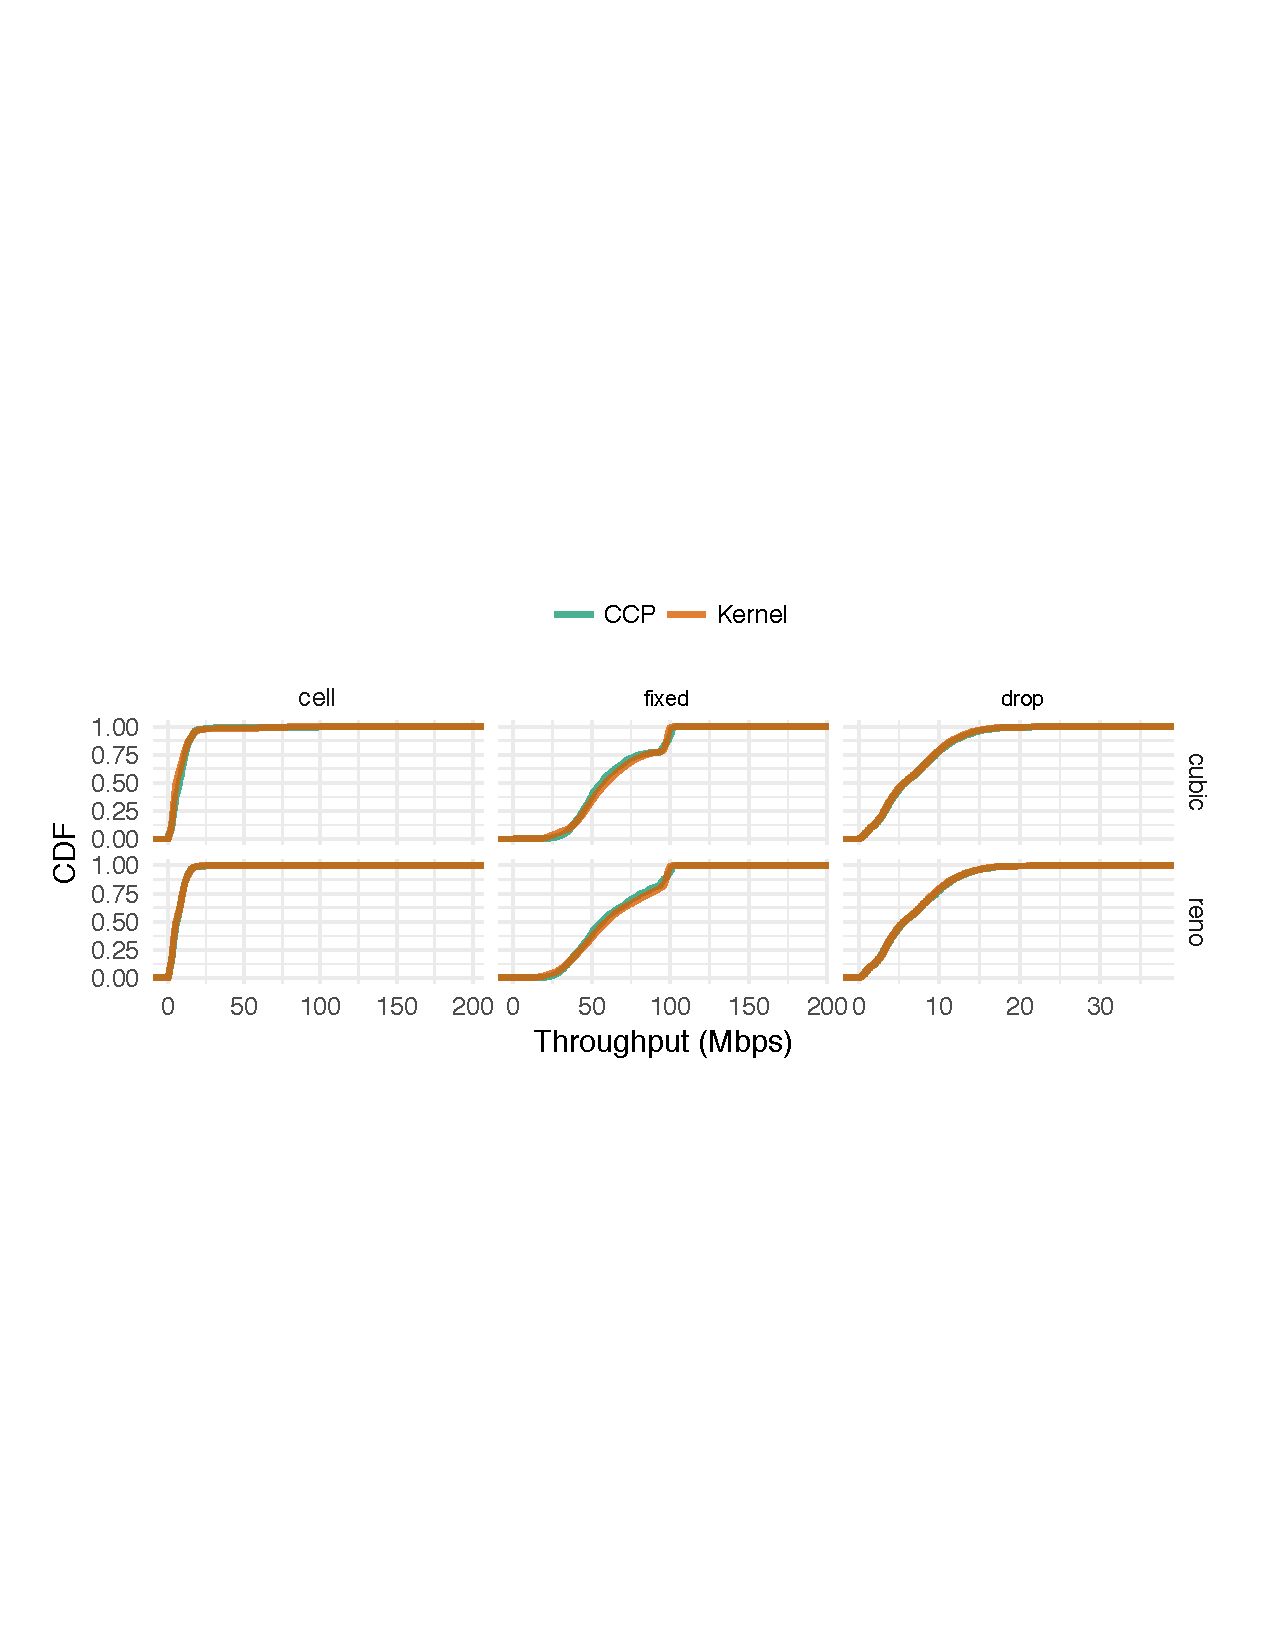
\includegraphics[width=\columnwidth]{img/throughput-cdf-flat}
\subcaption{Achieved throughput over 1 RTT periods. Note the different scales on the x-axes for the three scenarios.}\label{fig:eval:fidelity:tput-cdf}
\end{subfigure}
%
\begin{subfigure}{\columnwidth}
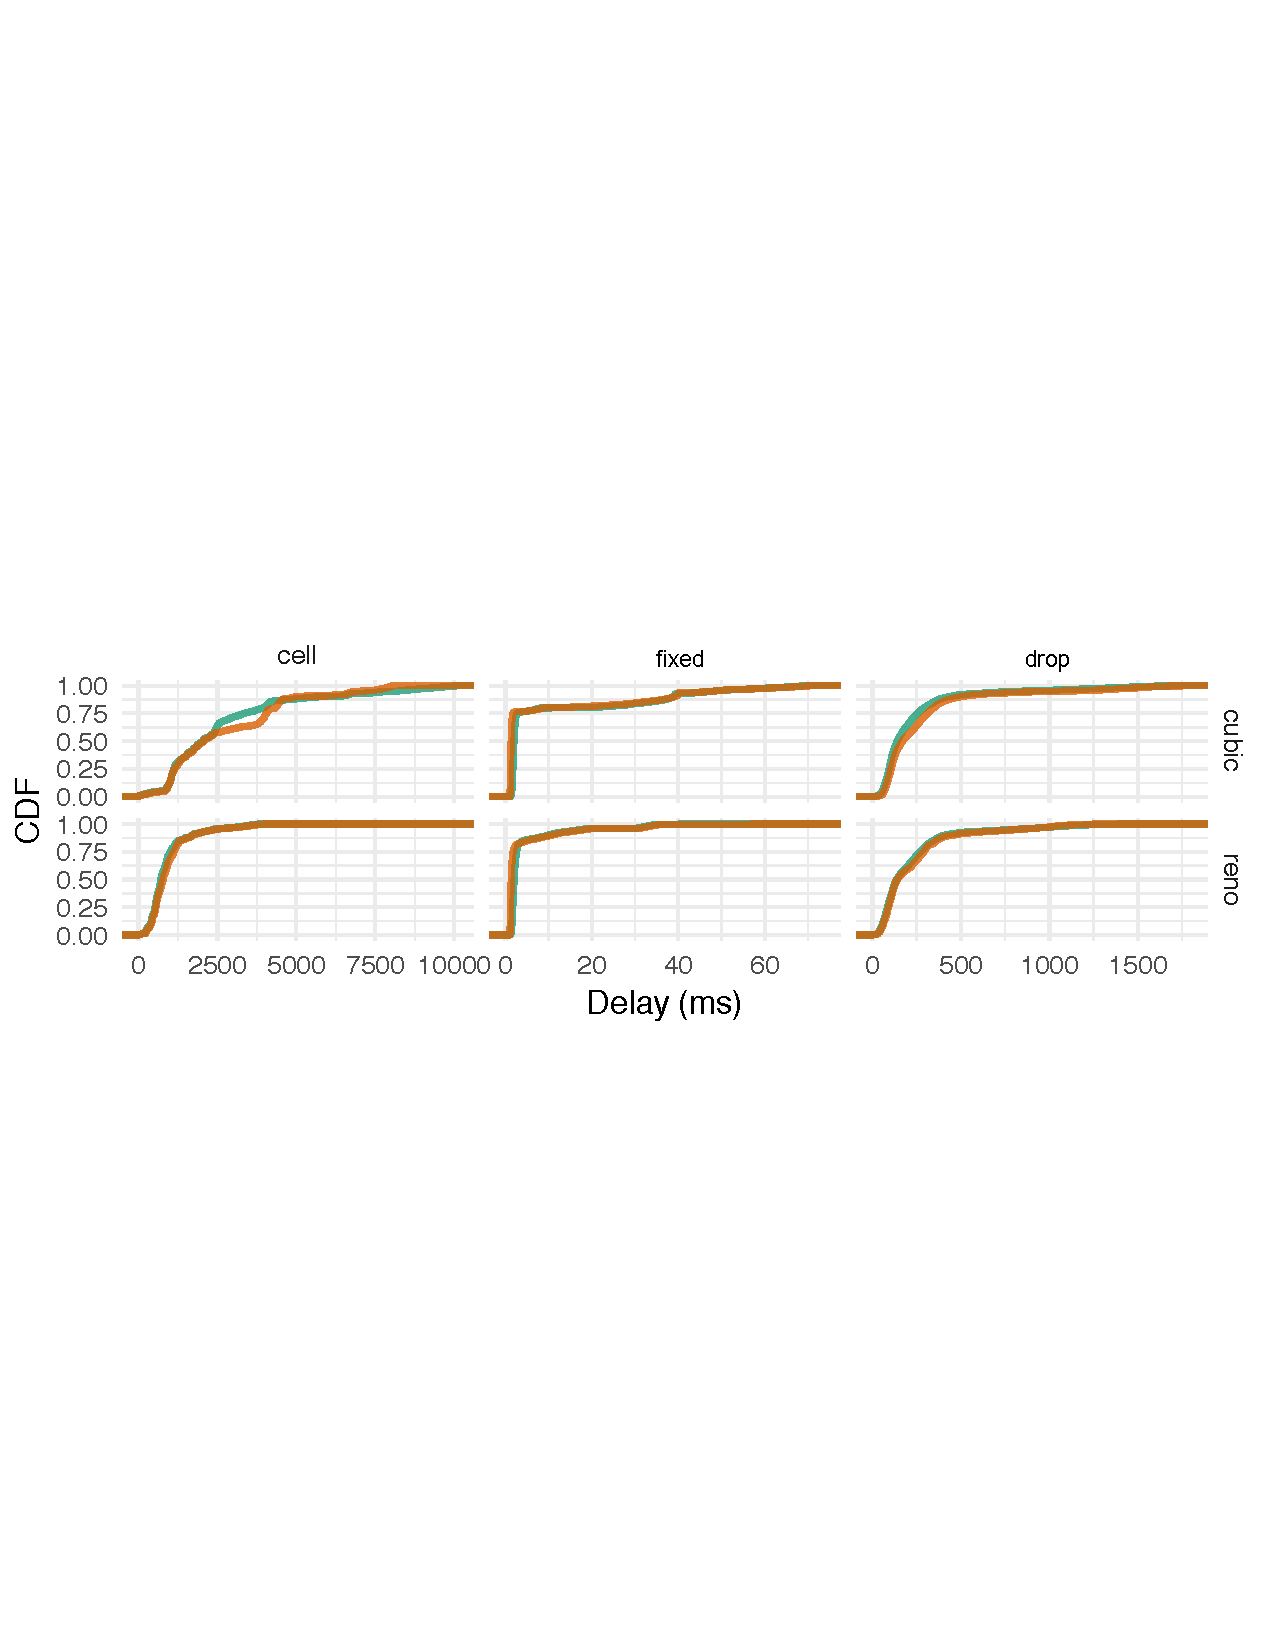
\includegraphics[width=\columnwidth]{img/delay-cdf-flat}
\subcaption{Achieved queueing delay over 1 RTT periods. Note the varying scales on the x-axes for the three scenarios.}\label{fig:eval:fidelity:delay-cdf}
\end{subfigure}
%
\caption{Comparison of achieved throughput over 20 ms periods. The achieved throughput distributions are nearly identical across the three scenarios and two congestion control algorithms evaluated.}\label{fig:eval:fidelity:cdfs-new}
\end{figure}

\bibliographystyle{abbrv}
\bibliography{ccp}
\end{sloppypar}

\end{document}
